\chapter{Einleitung}
\chaplabel{einleitung}
In dieser Arbeit wird der Prototyp eines Datenhandschuhs vorgestellt, der mit Sensoren die Finger- und Handbewegungen beim Schreiben auf einer Tastatur aufzeichnet und mittels geeigneter Methoden des maschinellen Lernens (ML) diese Bewegungen lernt, um später Tastendrücke aus den Bewegungen erkennen zu können. Dieses System soll die Tastatur als Eingabegerät ersetzen können.

Im folgenden Kapitel wird die Motivation zu diesem Projekt und der Aufbau der Arbeit erläutert. Außerdem wird der Projektumfang abgegrenzt.

\section{Motivation}
\seclabel{motivation}
In der heutigen Zeit sind Computer aus dem Alltag nicht mehr wegzudenken. In den meisten Fällen wird für die Eingabe von Befehlen eine Tastatur verwendet.

Für den Einsatz einer Tastatur sprechen viele Kriterien. Zum einen ist die Nutzung relativ schnell zu erlernen. Anfangs ist die Eingabegeschwindigkeit zwar oft nicht sonderlich hoch, jedoch wird diese mit einem gewissen Grad an Erfahrung und dem richtigen Schreibsystem rasch verbessert.

Hinzu kommt, dass die Tastatur sehr präzise in ihren Eingaben ist. Wenn eine Taste gedrückt wird, ist eine Fehlinterpretation des Computers nicht möglich. Sofern also das Tippen beherrscht wird, ist eine schnelle und stabile Kommunikation mit dem Computer gewährleistet.

Ein weiterer Grund für die Nutzung einer Tastatur ist, dass sie in der Produktion ausgesprochen günstig ist. Kaum eine andere Eingabemethode kommt an dieses Preis-Leistungs-Verhältnis heran.

Es gibt jedoch auch viele Gründe, die gegen die Verwendung einer Tastatur sprechen. Eine Tastatur ist beispielsweise relativ schlecht an motorische Fähigkeiten anpassbar. Mit weniger als 10 Fingern wird das Abdecken jeder Taste erschwert, wodurch die Effektivität negativ beeinflusst werden kann.

Außerdem ist eine Tastatur kaum an die Aufgabendomäne anpassbar. Die vorgegebenen Tasten und deren Anordnungen können nach der Herstellung nicht mehr verändert werden und das Ändern von Tastenbelegungen ist nur in bedingtem Maße nützlich. Sogenannte ,,Short-Cuts'', welche es ermöglichen bestimmte Funktionalitäten auf eine Kombination zwei oder mehrerer Tasten zu legen, reduzieren die Einschränkungen lediglich in geringem Umfang.

Das wahrscheinlich größte Problem mit konventionellen Tastaturen ist wohl der ergonomische Aspekt. Das Schreiben an einer Tastatur bietet einen sehr kleinen Spielraum für die Position der Hände. Der Mensch muss sich mit seiner gesamten Haltung an diese Position anpassen. Dies fördert diverse gesundheitliche Probleme, wie zum Beispiel das Repetitive-Strain-Injury-Syndrom \citep{disorders}.

In Anbetracht dieser Nachteile ist es schwer nachvollziehbar, dass an der Tastatur in den letzten Jahrzehnten kaum Veränderungen vollzogen wurden, und das, obwohl die Endgeräte, für welche die Tastatur benötigt wird, sich drastisch verändert haben.

Die Tastatur ist noch immer eng an das Layout einer Schreibmaschine angelehnt. Es wurden zwar verschiedene Anpassungen gemacht, wie zum Beispiel das Aufteilen der Tasten in zwei Hälften bei manchen Tastaturen, um die Handposition beim Schreiben zu verbessern, die Anordnung der Tasten im Ganzen sind jedoch kaum verändert.

Da die Geräte jedoch immer kleiner werden, ist die Tastatur nun oft der einschränkende Faktor. Bei Smartphones wird die virtuelle Tastatur oft nur noch mit zwei Finger bedient, der benötigte Platz umfasst jedoch trotzdem knapp den halben Bildschirm und ist somit nicht unerheblich.

% Das Ziel dieser Arbeit ist es, eine nicht-einschränkende Eingabemöglichkeit für Computer zu entwickeln, welche es ermöglicht Eingaben mit möglichst geringer Verzögerung an den Computer zu übermitteln und hierbei die Vorteile einer Tastatur nicht zu vernachlässigen.
\section{Vision}

\begin{figure}
    \centering
    \fbox{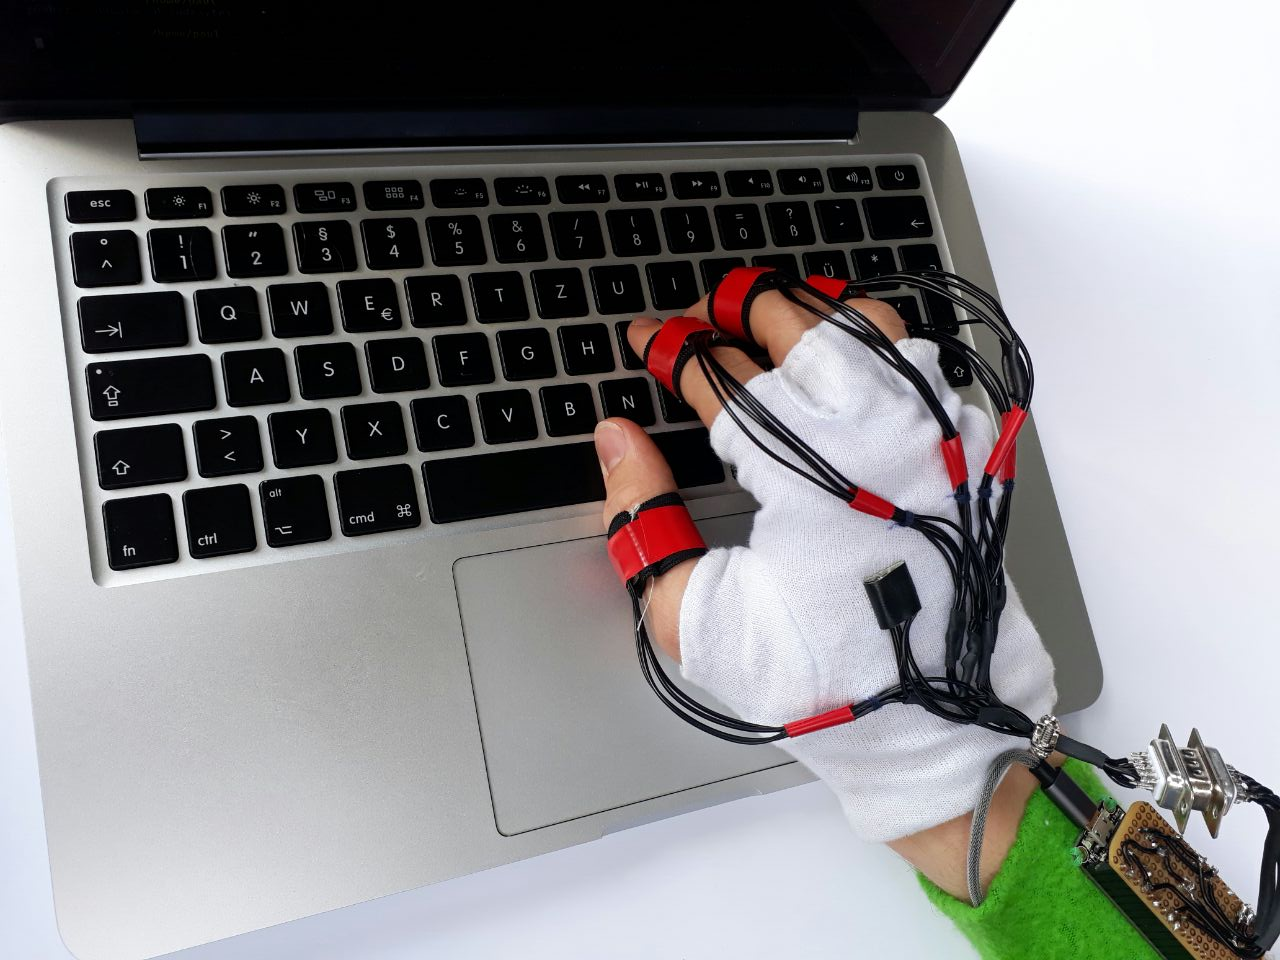
\includegraphics[width=0.98\textwidth]{../common/images/glove_laptop}}
    \caption[Datenhandschuh beim Aufzeichen der Lerndaten]{Der fertiggestellte Datenhandschuh während des Aufzeichnens der Lerndaten. Zu sehen sind die mit Gummiband befestigten Finger-IMUs, die Hand-IMU seitlich auf dem Handrücken sowie der Mikroprozessor mit Platine, welche auf einem Armband befestigt sind.}
    \figlabel{glove_laptop}
\end{figure}

Mit diesem Projekt wollen wir\footnote{In dieser Arbeit verwende ich die erste Person Singular, um mich auf meine eigene Arbeit zu beziehen, und die erste Person Plural, um auf Entscheidungen innerhalb des Projekts einzugehen.} einen Datenhandschuh entwickeln, welcher die herkömmliche Tastatur ersetzen kann. Mithilfe des Handschuhs soll es möglich sein, in jeder Position flüssig zu schreiben, ohne an hardwarebedingte Vorgaben gebunden zu sein. Dies soll ein deutlich ergonomischeres Schreiben ermöglichen, bei dem die Haltung der Person, welche den Datenhandschuh nutzt, nicht mehr an die Tastatur angepasst werden muss. Somit ist ein regelmäßiges Ändern der Schreibposition möglich, ebenso wie das Schreiben an verschiedenen Orten, an denen die Verwendung einer Tastatur eher unpraktisch oder kaum möglich wäre. Beispielsweise soll es möglich sein, den Handschuh im Stehen (ohne einen Tisch vor sich zu haben), im Liegen oder unterwegs zu benutzen.

Zu der Positionsunabhängigkeit kommt hinzu, dass auch die Bewegungen für die verschiedenen Eingaben unabhängig von externen Vorgaben sind. Jede Person kann ein eigenes Schreibsystem entwickeln und für sie wichtige Funktionalitäten, die mit einer Tastatur nur über Short-Cuts zu ermöglichen wären, mit eigenen Bewegungen belegen. Dadurch entsteht ein Eingabegerät, das in sehr vielen verschiedenen Kontexten verwendet werden kann.

Anforderungen an den Handschuh sind unter anderem, dass er robust und möglichst universal gebaut sein sollte, so dass er verschiedenen Hand\-typen passt. Die Kosten für die Herstellung sollten möglichst gering sein, um eine eventuelle Vermarktung zu ermöglichen und das Produkt für viele Nutzer attraktiv zu machen.

Die Daten, mit deren Hilfe die Bewegungsabläufe gelernt werden sollen, werden mithilfe einer Tastatur aufgezeichnet. Dies ermöglicht, dass Nutzer des Datenhandschuhs die bereits im Muskelgedächtnis gespeicherten Bewegungen für verschiedene Tasten nutzen können und sich nicht für jede Tastatureingabe eine Bewegung ausdenken müssen.

Nach dem Lernen soll auf die Tastatur verzichtet werden können. Anhand der Sensor- und Tastaturdaten soll ein maschineller Lernalgorithmus in der Lage sein, die Fingerbewegungen den dazugehörigen Tasten zuordnen zu können.

\section{Umfang und Abgrenzung der Arbeit}
\seclabel{umfang}

Das Projekt ist im Rahmen zweier Bachelorarbeiten entstanden. Da diese auf jeweils 5 Monate begrenzt sind, war es nicht möglich, die Vision vollständig umzusetzen.
Im Folgenden wird darauf eingegangen, auf welche Aspekte der Fokus gelegt wurde und welche Teile eventuell nur stark vereinfacht umgesetzt werden konnten.

Eine Vereinfachung ist, dass wir nur einen Handschuh gebaut haben, um sowohl Resourcen als auch Zeit zu sparen.
Desweiteren haben wir den Handschuh nicht auf mehrere, sondern lediglich auf eine Person ausgelegt und nicht für verschiedene Hand\-typen designed.

Die Voraussetzung für das Nutzen des Muskelgedächtnisses zum Schreiben auf einer Tastatur ist, dass die Person ein geübter Schreiber ist. Wir konzentrierten uns auf diesen Fall, damit die ohne Tastatur durchgeführten Bewegungen denen der Lernphase ähneln. Wir beachteten zunächst nicht den Fall, dass sich die Fingerbewegungen zu einer Taste von Fall zu Fall stark unterscheiden (wenn die Person die Taste etwa erst suchen muss).

Wir haben in diesem Projekt zudem nicht viele verschiedene ML-Methoden evaluiert, sondern lediglich 2 verschiedene neuronale Netze ausprobiert und uns für das Netz entschieden, welches sich für unser Projekt besser eignet. Je komplexer die Aufgabe wird, desto wahrscheinlicher ist es, dass weitere Methoden evaluiert werden müssen, das Projekt bietet also Raum für weitere Forschung.

Unser Projektziel kann in drei große Bereiche eingeteilt werden:

\begin{enumerate}
    \item Entwurf eines Systems zur Aufzeichnung der charakteristischen Handbewegungen beim Tippen sowie der dazugehörigen Tastatureingaben.
    \item Definition eines Ansatzes zum Rückschließen auf Tastatureingaben aus den aufgezeichneten Bewegungen unter der Verwendung von Verfahren des maschinellen Lernens.
    \item Bewertung der Qualität dieser Rückschlüsse und der Nutzbarkeit eines solchen Verfahrens als Alternative zur klassischen Tastatur.
\end{enumerate}

Der erste Teil, der Entwurf des Systems, ist Hauptbestandteil der Bachelorarbeit von Paul \citet{paul} und dort nachzulesen. Ich beschränke mich auf diese Aspekte lediglich, soweit sie die Verständlichkeit meiner Arbeit unterstützen.

Die vorliegende Arbeit behandelt die Nutzung von maschinellem Lernen zur Ermittlung von Tastendrücken anhand von aufgezeichneten Bewegungen. In beiden Arbeiten wird auf die Bewertung und die Analyse des Projektes eingegangen.

\section{Aufbau der Arbeit}
\seclabel{aufbau}
Diese Arbeit ist in mehrere Kapitel gegliedert. In \chapref{einleitung} wurde die Motivation für den erstellten Prototyp erläutert und ein Überblick über die Problematik der jetzigen Eingabemethode gegeben.

In \chapref{grundlagen} wird eine Grundlage über den für das Projekt relevanten Bereich des maschinellen Lernens geschaffen. Unter anderem wird der Unterschied von überwachtem und unüberwachtem Lernen erläutert, die in diesem Projekt verwendeten Typen eines neuronalen Netzes erklärt und auf die Problematik von unbalancierten Datensätzen eingegangen.

Im  Abschnitt ,,State of the Art', \chapref{state}, werden verwandte Projekte und Forschungsarbeiten aufgezeigt und diskutiert.
% Es wird auf verschiedene Eingabemethoden, wie zum Beispiel Sprach- und Gestenerkennung eingegangen.

Es folgt ein Kapitel über das angewandte Verfahren, welches die Bewegungsdaten extrahiert und mit ihrer Hilfe Tastendrücke erkennt. In diesem Kapitel wird der Datenhandschuh und die verwendeteten Bibliotheken beschrieben.  Zudem wird auf das Vorverarbeiten der Daten eingegangen und die zu Grunde liegende Netzwerkarchitektur mitsamt aller Kon\-fi\-gu\-ra\-tions\-mög\-lich\-kei\-ten erläutert.

In \chapref{evaluation} werden die Versuche beschrieben, welche für die Bewertung des Daten\-hand\-schuhs und des vorgestellten Verfahrens verwendet wurden, um dann auf deren Ausgang und die Schlüsse, die wir aus den Versuchen ziehen konnten, einzugehen.
% die Genauigkeit und Funktionalität des Datenhandschuhs innerhalb der einzelnen Experimente evaluiert. Zudem wird ein Fazit des gesamten Projekts gezogen.

Schließlich werden in \chapref{fazit} die Ergebnisse dieser Arbeit zusammengefasst und Verbesserungsmöglichkeiten und weitere mögliche Schritte aufgezeigt.



